\chapter{The Kronecker-Weber Theorem}
\label{cp:kw}
\section{General Idea}
Recall that,
\newtheorem*{restatement}{Theorem 1.1}
\begin{restatement}[Kronecker-Weber]
    ~\begin{center}
    Every abelian extension of $\mathbb{Q}$ is contained in a cyclotomic field.
\end{center}
\end{restatement}
\noindent
We will first presents the general idea towards the goal and leave technical details to remaining sections. The main structure of our proof here is built in favor of formalization and automated theorem proving, which emphasis computability and clarity.
\subsection{General Idea: Reducing to Wild Ramification}
    We first reduce the case into abelian extension $K/\mathbb{Q}$ \textbf{that only has wild ramification}. This is done by "turning every tame ramification one by one into unramified element".
    \begin{thm}
    \label{thm:thm-31}
    Suppose that $K/\mathbb{Q}$ is an abelian extension, $p$ is tamely ramified over $K$. Then we can construct another \textbf{abelian} extension $K'/\mathbb{Q}$, together with a subfield $L$ of some cyclotomic field, such that
    \begin{enumerate}
        \item $p$ is unramified in $K'$
        \item unramified prime in $K$ stays unramified in $K'$
        \item $LK=LK'$
    \end{enumerate}
    \end{thm}
    \begin{wrapfigure}{r}{0.45\textwidth}
    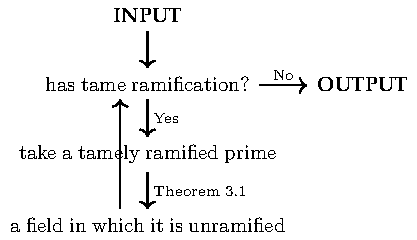
\includegraphics[width=\linewidth]{Figures/figure4.pdf}
    \end{wrapfigure}
    \noindent
    This theorem induces an algorithm as shown on the right.
    We claim that \textbf{after finite steps of iteration, the algorithm will halt and we will get a field with only wildly ramified primes}. As drawn below, the fate of tamely ramified prime and unramified prime under the algorithm is destined - tamely ramified prime must be turned to unramified, whereas unramified must stay still. The only variant here is wildly ramified primes.
    \begin{center}
    \begin{tikzcd}[sep=small]
	tamely &&& unramified \\
	\\
	\\
	wildly
	\arrow[from=1-1, to=1-4]
	\arrow[from=1-4, to=1-4, loop, in=55, out=125, distance=10mm]
	\arrow[dashed, from=4-1, to=1-1]
	\arrow[dashed, from=4-1, to=1-4]
	\arrow[dashed, from=4-1, to=4-1, loop, in=305, out=235, distance=10mm]
    \end{tikzcd}
    \end{center}
    According to \autoref{thm:thm-24}, there are only finitely many ramified primes. Viewing tame and wild ramification in the graph as a whole (imagine drawing a box around them). We shall notice that there are no arrows pointing to the box, only arrows pointing out (nothing get converted into ramified prime).\\
    This means that whatever happends, the number of primes in the box is strictly decreasing - this decrease must halt within finite step since the number is finite. Thus the algorithm is halting. And since the process can go on as long as there exists a tamely ramified prime, it must leaves a field with only wild ramification when it halts.\\
    Suppose the process ends with field $\mathscr{K}$, we claim that \textbf{if $\mathscr{K}$ is contained in a cyclotomic field, then so is $K$}. In fact, if we denote the field obtained at step $n$ as $K_n$ and $L_n$, we can assert that,
    \begin{center}
        $K_n$ is contained in a cyclotomic field $\Rightarrow$ so is $K_{n-1}$
    \end{center}
    This is because if $K_n$ is contained in $\mathbb{Q}(\zeta_m)$, $L_n$ is contained in $\mathbb{Q}(\zeta_w)$, then $L_n K_n$ is contained in $\mathbb{Q}(\zeta_{mw})$. Since $L_n K_n = L_n K_{n-1}$, we have $K_{n-1} \leq L_n K_{n-1} \leq \mathbb{Q}(\zeta_{mw})$.
    \begin{center}
    \begin{tikzcd}[sep=small]
	& \textcolor{rgb,255:red,214;green,92;blue,92}{\mathbb{Q}(\zeta_{mw})} \\
	{\mathbb{Q}(\zeta_m)} &&& {\mathbb{Q}(\zeta_w)} \\
	& \textcolor{rgb,255:red,214;green,92;blue,92}{L_n K_n} & \textcolor{rgb,255:red,214;green,92;blue,92}{L_n K_{n-1}} \\
	{K_{n}} && \textcolor{rgb,255:red,214;green,92;blue,92}{K_{n-1}} & {L_n}
	\arrow[no head, from=2-1, to=1-2]
	\arrow[no head, from=2-1, to=4-1]
	\arrow[no head, from=2-4, to=1-2]
	\arrow[no head, from=2-4, to=4-4]
	\arrow[color={rgb,255:red,214;green,92;blue,92}, no head, from=3-2, to=1-2]
	\arrow[color={rgb,255:red,214;green,92;blue,92}, Rightarrow, dotted, no head, from=3-2, to=3-3]
	\arrow[no head, from=4-1, to=3-2]
	\arrow[color={rgb,255:red,214;green,92;blue,92}, no head, from=4-3, to=3-3]
	\arrow[dotted, harpoon, from=4-3, to=4-1]
	\arrow[dotted, harpoon', from=4-3, to=4-4]
	\arrow[no head, from=4-4, to=3-2]
	\arrow[no head, from=4-4, to=3-3]
\end{tikzcd}
    \end{center}
    Then we can use reverse induction to prove the lemma. Then we shall presents the following algorithm for proving "contained in a cyclotomic field",
    \begin{importantbox}
    \begin{enumerate}
        \item[\textbf{INPUT}] An abelian extension $K/\mathbb{Q}$.
        \item[\textbf{STEP 1}] Run $K$ through the algorithm induced by \autoref{thm:thm-31}.
        \item[\textbf{STEP 2}] STEP 1 halts with an abelian extension $\mathscr{K}/\mathbb{Q}$ which has only wild ramification.
        \item[\textbf{STEP 3}] Prove that $\mathscr{K}$ is contained in a cyclotomic field.
        \item[\textbf{OUT}] Thus $K$ is contained in a cyclotomic field.
    \end{enumerate}
    \end{importantbox}
    \noindent
    Which finishes our first reduction.
\subsection{General Idea: Reducing to Prime Power Cyclic Extension}
Next we reduce the case into abelian extension $K/\mathbb{Q}$ \textbf{such that $[K : \mathbb{Q}] = p^n$ for some $p$ and $n$}.

\begin{wrapfigure}{l}{0.4\textwidth}
    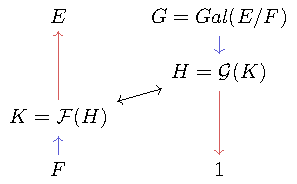
\includegraphics{Figures/figure5.pdf}
\end{wrapfigure}
\noindent
Recall that by abelian, we mean $[K : \mathbb{Q}]$ is finite and $Gal(K/\mathbb{Q})$ is abelian. Also recall the famous Galois fundamental theorem that establishes connection between Galois group and corresponding subfields.
% \[\begin{tikzcd}[sep=tiny]
% 	E && {G=Gal(E/F)} \\
% 	\\
% 	&& {H=\mathcal{G}(K)} \\
% 	{K=\mathcal{F}(H)} \\
% 	\\
% 	F && 1
% 	\arrow[color={rgb,255:red,92;green,92;blue,214}, from=1-3, to=3-3]
% 	\arrow[color={rgb,255:red,214;green,92;blue,92}, from=3-3, to=6-3]
% 	\arrow[color={rgb,255:red,214;green,92;blue,92}, from=4-1, to=1-1]
% 	\arrow[tail reversed, from=4-1, to=3-3]
% 	\arrow[color={rgb,255:red,92;green,92;blue,214}, from=6-1, to=4-1]
% \end{tikzcd}\]
\newline
$E/F$ is a finite Galois extension, $F \leq K \leq E$ and $H \leq G$. $K$ is the fixed field of $H$, denoted $K=\mathcal{F}(H)$. $H$ is the fixing group of $K$, denoted $H=\mathcal{G}(K)$. $\mathcal{F}$ and $\mathcal{G}$ are inclusion-reversing bijections, meaning $H$ descends as $K$ moves up. And the segment with same color shares same index. $E/K$ is always Galois, whereas $K/F$ is Galois iff $H \lhd G$.
\begin{listing}[!htpb]
\begin{minted}[escapeinside=+-]{lean}
def IsGalois.intermediateFieldEquivSubgroup {F : Type u_1} [Field F] {E : Type u_2} [Field E] [Algebra F E] [FiniteDimensional F E] [IsGalois F E] :
IntermediateField F E +$\simeq_o$- (Subgroup (E +$\simeq_a$-[F] E))+$^{od}$-
\end{minted}
\end{listing}
\newline
Thus $\mid Gal(K/\mathbb{Q}) \mid = [K : \mathbb{Q}]$ is finite. Therefore we can use the structure theorem of finite abelian group to break $Gal(K/\mathbb{Q})$ into product of prime power groups.
\begin{listing}[!htpb]
\begin{minted}[escapeinside=||]{lean}
theorem AddCommGroup.equiv_directSum_zmod_of_finite (G : Type u) [AddCommGroup G] [Finite G] : 
    |$\exists$| (|$\iota$| : Type) (x : Fintype |$\iota$|) (p : |$\iota$| → |$\mathbb{N}$|) (_ : |$\forall$| (i : |$\iota$|), Nat.Prime (p i)) 
    (e : |$\iota$| → |$\mathbb{N}$|),
Nonempty (G |$\simeq_+$| DirectSum |$\iota$| fun (i : |$\iota$|) => ZMod (p i ^ e i))
\end{minted}
\end{listing}
\newline
Then we may reconstruct $K$ as the composition of corresponding fixed field of those prime power group. To do that, we need another property stated in fundamental Galois theorem,
\begin{thm}
    \label{thm:thm-32}
    Given finite Galois extension $K/F$, if $H_1, \ H_2 \leq Gal(K/F)$, then
    \begin{equation}
    \notag
    \mathcal{F}(H_1 \sqcap H_2) = \mathcal{F}(H_1) \sqcup \mathcal{F}(H_2), \ \mathcal{F}(H_1 \sqcup H_2) = \mathcal{F}(H_1) \sqcap \mathcal{F}(H_2)
    \end{equation}
\end{thm}
\noindent
In particular, the following algorithm to disassemble $K$ into composition of prime power degree abelian extension of $\mathbb{Q}$ can be established,
\begin{importantbox}
\begin{enumerate}
	\item[\textbf{INPUT}] An abelian extension $K$.
	\item[\textbf{STEP 1}] Decompose $Gal(K/\mathbb{Q})$ into $\mathbb{Z}_{p_1^{r_1}} \times \dots \times \mathbb{Z}_{p_n^{r_n}}$.
	\item[\textbf{STEP 2}] For every $\mathbb{Z}_{p_i^{r_i}}$ (denoted as $Z_i$), denote $\prod_{j \neq i} Z_j$ as $A_i$,
        \begin{enumerate}
        \item[1.] Since $Gal(K/\mathbb{Q})$ is abelian, $A_i \lhd Gal(K/\mathbb{Q})$. (Strictly speaking, $A_i$ is a subgroup of $Gal(K/\mathbb{Q})$ up to isomorphic)
        \item[2.] According to Galois theory, $\mathcal{F}(A_i)/\mathbb{Q}$ is Galois.
        \end{enumerate}
    \item[\textbf{STEP 3}] By \autoref{thm:thm-32}, $\mathcal{F}(\sqcap A_i) = \sqcup \mathcal{F}(A_i)$. $\sqcap A_i = {1}$, hence $\mathcal{F}(\sqcap A_i) = K = \sqcup \mathcal{F}(A_i)$.
    \item[\textbf{STEP 4}] Each of $\mathcal{F}(A_i)$ is of prime power degree since $[\mathcal{F}(A_i) : \mathbb{Q}] = |Gal(K/\mathbb{Q})/A_i| = p_i^{r_i}$.
    \item[\textbf{STEP 5}] Each of $\mathcal{F}(A_i)$ is abelian since its Galois group is exactly $A_i = \prod_{j \neq i} \mathbb{Z}_{p_i^{r_i}}$.
    \item[\textbf{OUT}] The decomposition $\sqcup \mathcal{F}(A_i)$.
\end{enumerate}
\end{importantbox}
\subsection{General Idea: Finishing Proof}
Now suppose we've got,
\begin{thm}
\label{thm:thm-33}
Given an abelian extension $K/\mathbb{Q}$ with $[K : \mathbb{Q}]=p^n$ for some $p$ and $n$, if every prime other than $p$ is unramified, then
\begin{itemize}
\item if $p \neq 2$, then $K$ is contained in $\mathbb{Q}({\zeta_{p^{n+1}}})$
\item if $p=2$, then $K$ is contained in $\mathbb{Q}(\zeta_{2^{m+2}})$ for some $m$
\end{itemize}
\end{thm}
\noindent
Then we can combine two algorithms given above and build the final algorithm towards the Kronecker-Weber theorem,
\begin{importantbox}
\begin{enumerate}
\item[\textbf{INPUT}] An abelian extension $K$.
\item[\textbf{STEP 1}] Run $K$ through the algorithm induced by \autoref{thm:thm-31}, this halts with an abelian extension $\mathscr{K}$ which has only wildly ramified primes.
\item[\textbf{STEP 2}] Run $\mathscr{K}$ through the decomposition algorithm, this gives $\mathscr{K} = \sqcup K_i$, where $K_i$ are prime power degree abelian extensions.
\item[\textbf{STEP 3}] For every $K_i$,
\begin{enumerate}
\item Since $\mathscr{K}$ has no tamely ramified prime, $K_i$ must also have no tame ramification.
\item Suppose $[K_i : \mathbb{Q}]=p^n$, then for any prime $q \neq p$, $q$ must be either tamely ramified or unramified. 
\item Thus by (a), the only wildly ramified prime in $K_i$ is $p$.
\item Thus by \autoref{thm:thm-33}, $K_i$ is contained in cyclotomic field.
\end{enumerate}
\item[\textbf{STEP 4}] Since the composite of cyclotomic fields is cyclotomic, $\mathscr{K}$ is contained in a cyclotomic field.
\item[\textbf{OUT}] $K$ is contained in a cyclotomic field.
\end{enumerate}
\end{importantbox}
\newpage
\section{Reducing to Wildly Ramified Case}
In this section we prove \autoref{thm:thm-31},
\newtheorem*{restatementa}{Theorem 3.1}
\begin{restatementa}
    Suppose that $K/\mathbb{Q}$ is an abelian extension, $p$ is tamely ramified over $K$. Then we can construct another \textbf{abelian} extension $K'/\mathbb{Q}$, together with a subfield $L$ of some cyclotomic field, such that
        \begin{enumerate}
            \item $p$ is unramified in $K'$
            \item unramified prime in $K$ stays unramified in $K'$
            \item $LK=LK'$
        \end{enumerate}
\end{restatementa}
\begin{proof}(\textcolor{red}{\textbf{SKETCH}})
~\begin{enumerate}
\item Constructing $K'$\\
    $I_1$ is trivial by Theorem 2.5. Then by Theorem 2.6, $I_0/I_1 = I_0 \leq (k(p))^\times = (\mathbb{Z}_p)^\times$. Thus $e \mid p-1$. Notice that $(\mathbb{Z}_p)^\times \simeq Gal(\mathbb{Q}(\zeta_p)/\mathbb{Q})$, then by Galois theory, $L = \mathcal{F}(I_0) \leq \mathbb{Q}(\zeta_p)$ has degree $e$ over $\mathbb{Q}$.
    \\
    \noindent
    It can be proved that $p$ is totally ramified in $\mathbb{Q}(\zeta_p)$. $e \mid p - 1$ then $e$ is relatively prime to $p$, and so $p$ is tamely ramified in $\mathbb{Q}(\zeta_p)$. Hence $p$ is totally and tamely ramified in $L$. Thus there is a unique prime $\mathfrak{p}$ in $L$ that lies over $p$. Then take $\mathfrak{P}$ a prime of $LK/L$ lying over $\mathfrak{p}$. So $\mathfrak{P}$ lies over $p$. Let $I'_0 = I_0(\mathfrak{P}/p)$ and $K' = \mathcal{F}(I'_0)$ the fixed field.
    \begin{figure}[!htpb]
    \centering
    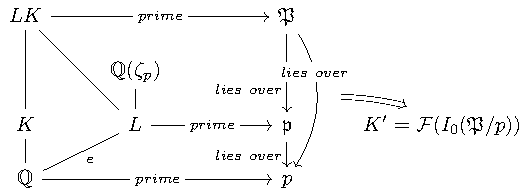
\includegraphics[width=0.6\linewidth]{Figures/figure6.pdf}
    \end{figure}
\item $p$ is unramified in $K'$ whereas unramified prime stays unramified\\
    $L$ is ramified only at $p$, then $q$ remains unramified in $L$  as long as $q$ is unramified in $K$ and $q \neq p$. Consequently, $q$ is unramified in the extension $LK$. Therefore, if $q$ is unramified in $K$, it will also be unramified in $K' \leq LK'$. Additionally, $p$ remains unramified in $K'$ since $K'$ is the inertial field of $\mathfrak{P}/p$.
\item $LK=LK'$
    \begin{itemize}
    \item $[LK' : K'] \geq e$:\\
        $p$ is unramified in $K'$ and $p$ is totally ramified in $L$ with ramification $e = [L : \mathbb{Q}]$ so $p$ ramified in $LK'$ with ramification index $e$, by Theorem 2.1, $e \mid [LK':K']$, thus $[LK' : K'] \geq e$.
    \item $e \geq [LK : K'] \geq [LK' : K']$:\\
        $[LK : K'] = |I'_0|$ according to the setup. $\mathfrak{P}$ is tamely ramified since $p$ is tamely ramified in both $L$ and $K$. By Theorem 2.6, $I'_0 \leq (k(p))^\times = (\mathbb{Z}_p)^\times$, so $I'_0$ is a cyclic group. Similarly, $Gal(LK/\mathbb{Q})$ injects into $Gal(K/\mathbb{Q}) \times Gal(L/\mathbb{Q})$ and so $I'_0$ does as well.\\
        Let $\mathfrak{p}' = \mathfrak{P} \cap K$. Then by definition, $I'_0$ restricted to $K$ gives an element in the inertia group $I_0(\mathfrak{p}'/p)$ but $\mathfrak{p}'$ is conjugate to $\mathfrak{p}$ so the order of $I_0(\mathfrak{p}'|p)$ is $|I_0| = e$.\\
        Thus $I'_0$ lives in the subgroup $I_0(\mathfrak{p}'|p) \times \text{Gal}(L/\mathbb{Q})$, both of which are groups of order $e$ so $I'_0$ has exponent $e$. Since it is cyclic and of exponent $e$, $|I'_0| \leq e$.
    \end{itemize}
    Thus $e \geq |I'_0| = [LK : K'] \geq [LK' : K'] \geq e$. Hence $[LK : K'] = [LK' : K']$, $LK = LK'$.
\end{enumerate}


\end{proof}
\section{Reducing to Prime Power Cyclic Extension}
In this section we prove Theorem 3.3,
\newtheorem*{restatementb}{Theorem 3.3}
\begin{restatementb}
Given an abelian extension $K/\mathbb{Q}$ with $[K : \mathbb{Q}]=p^n$ for some $p$ and $n$, if every prime other than $p$ is unramified, then
\begin{itemize}
\item if $p \neq 2$, then $K$ is contained in $\mathbb{Q}({\zeta_{p^{n+1}}})$
\item if $p=2$, then $K$ is contained in $\mathbb{Q}(\zeta_{2^{m+2}})$ for some $m$
\end{itemize}
\end{restatementb}
\begin{proof}(\textcolor{red}{\textbf{SKETCH}})
~\begin{enumerate}
\item $p \neq 2$ ($p$ is odd):\\
    The Galois group $Gal(\mathbb{Q}(\zeta_{p^{n+1}})/\mathbb{Q})$ is cyclic of order $p^n(p - 1)$. Let $L$ be the unique subextension of degree $p^n$. Then, $Gal(L/\mathbb{Q})$ is cyclic of order $p^n$.

    Consider the compositum $LK$. Let $\sigma$ be a generator of $Gal(L/\mathbb{Q})$, and let $\tau$ be a lift of $\sigma$ to $Gal(LK/\mathbb{Q})$. Let $F$ be the fixed field of $\langle \tau \rangle$. Since $\sigma$ generates $Gal(L/\mathbb{Q})$, the fixed field of $\sigma$ is $\mathbb{Q}$, implying $L \cap F = \mathbb{Q}$. Hence, $Gal(LK/\mathbb{Q})$ embeds into $Gal(L/\mathbb{Q}) \times Gal(K/\mathbb{Q})$, and $\tau$ has order exactly $p^n$.
        
    Thus, $[LK : F] = p^n$, and since $L \cap F = \mathbb{Q}$, it follows that $LK = L$. Therefore, $K \subset L \subset \mathbb{Q}(\zeta_{p^{n+1}})$, proving the first part.
\item $p = 2$:\\
    For $p = 2$, we reduce to the case where $K/\mathbb{Q}$ is a cyclic $2^n$-extension with discriminant a power of $2$. Consider $K(i)$, where $i = \sqrt{-1}$. Then $K(i)$ is unramified away from $2$. Let $K'$ be the fixed field of complex conjugation in $K(i)$. Then $K'$ is totally real of degree $2^m$ with discriminant a power of $2$ and is cyclic. Take $L = \mathbb{Q}(\zeta_{2^{m+2}}) \cap \mathbb{R}$, the real subfield of $\mathbb{Q}(\zeta_{2^{m+2}})$. Since $K'$ and $L$ are both totally real and cyclic of the same degree, $K' = L$.
    Finally, since $K \subset K(i) = K'(i) \subset \mathbb{Q}(\zeta_{2^{m+2}}, i)$ and the latter is cyclotomic, the proof is complete.
\end{enumerate}
\end{proof}